\section{L'entreprise}

On verra que le producteur pour atteindre ses objectifs veut maximiser ses profits. Pour atteindre cet objectif il procéde en deux étapes, en premier lieu il optimise la gestion des ressources pour une niveau de production donné (minimisation des coûts). Ensuite il optimise son niveau de production en maximisant ses profits.

\subsection{Le programme de minimisation des coûts}

$$
\left\{
\begin{array}{cc}
 min_{R_i}C= & \sum_i p_iR_i  \\
 sc: & \\
 &\bar{Q} \leq F(R_i)\\
 & 0\leq R_i \ \forall i \in \{ 1,..n .\}
\end{array} 
\right.
$$
Les choix optimaux nous indiquent que le taux marginal de substitution est égal au rapport des prix $\frac{p_i}{p_j}$, en effet \textbf{le coût de substitution du bien i par le bien j doit être égal à son gain.}\\

\subsection{Le programme de maximisation des profits}


$$
\left\{
\begin{array}{cc}
 max_{Q,R_1..R_n}(\pi ) = & p_Q Q -\sum_i p_iR_i  \\
 sc: & \\
 & Q \leq F(R_i)\\
 & 0\leq R_i \ \forall i \in \{ 1,..n .\}
\end{array} 
\right.
$$

La résolution du programme nous indique que les productivités marginales doivent être égales à leur prix:
$$ \partial_{R_i} F = \frac{p_{R_i}}{p_Q}
$$

\subsection{Fonction de coût}

 On utilise la relation $TMS_{i,j}=\frac{p_j}{p_i}$ pour isoler les $R_i$ en fonction de $ Q$ et ainsi obtenir $C=F(Q,p_1,..,p_n)$
\subsection{Fonction d'offre}

Généralement on calcule $ \frac{\partial \pi}{\partial Q}=0$ et on isole $Q$. Cependant s'il y a dépendance linéaire entre $\pi$ et $Q$, on obtiens de la méthode précédente le prix $p=p^*$ auquel l'offre est parfaitement élastique. On a \textbf{dans ce cas là}:
$$
\left\{
\begin{array}{cc}
\infty & p>p^* \\
\left[0,\infty\right[ & p=p^* \\
0 & p<p^*
\end{array} 
\right.
$$

\subsection{La fonction de production}

On parle de fonction de production pour désigner la relation entre les entrées et les sorties de la production:
$$
S=F(E_1,...E_n)
$$
On définit ainsi le taux de substitution technique :
$$
TST_{i,j}=\frac{\partial_{E_j} F}{\partial_{E_i} F}
$$
Une autre fonction importante est la frontière de production. Elle se construit analytiquement en saturant les contraintes sur les entrée i.e $E_1+..E_n=M$ et en exprimant $\phi (S_1,..,S_n)=0$. On peut ainsi définir le taux de transformation de production $TTP_{i,j}=\frac{\partial_{S_j} \phi}{\partial_{S_i} \phi}$.\\
On peut aussi construire cette fonction géométriquement en unissant les points de tangence entre les points de tangence des fonctions de production, on obtiens un homologue à la courbe des contrats pour la production que l'on va visualiser dans un nouveau système cartésien $(O,S_1,S_2)$


\begin{figure}[h]
\begin{center}
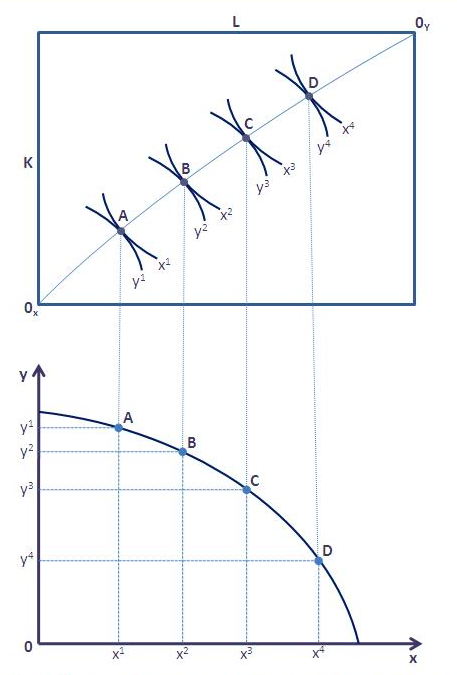
\includegraphics[scale=0.3]{./img/IM3}
\caption{Obtention frontière de production}
\end{center}
\end{figure}